\section{Algebra}
\subsection{Coordinate Geometry}

\begin{problem}
    For what values of \(a, b, c\) does the circle \(x^2 - 2ax + y^2 - 2by + c = 0\) contain the origin?
\end{problem}

\begin{solution}
    Note that the original equation to be simplified as
    \[
        \para{x - a}^2 + \para{y - b}^2 = a^2 + b^2 - c,
    \]
    and for this to contain the point \(\para{x, y}\), we need to have
    \[
        \para{x - a}^2 + \para{y - b}^2 < a^2 + b^2 - c.
    \]

    Putting in \(\para{x, y} = \para{0, 0}\) gives
    \[
        a^2 + b^2 < a^2 + b^2 - c
    \]
    which gives \(c < 0\).
\end{solution}

\subsection{Equations}
\begin{problem}
    For what values of \(a\) does the equation \(ax^2 - x + 1 = 0\) have two real roots? Explain the behaviour of the roots as \(a \to 0_{\pm}\).
\end{problem}

\begin{solution}
    When \(a = 0\), this equation has one root \(x = 1\).

    When \(a \neq 0\), this equation is a quadratic indeed, and we have
    \begin{align*}
        \Delta = 1 - 4a > 0
    \end{align*}
    so \(a < \frac{1}{4}\).

    We recall the quadratic formula for \(ax^2 + bx + c = 0\) as
    \[
        x_{1, 2} = \frac{-b \pm \sqrt{b^2 - 4ac}}{2a}
    \]
    for \(a \neq 0\).

    Alternatively, we can transform the original equation to \(c \para{\frac{1}{x}}^2 + b \para{\frac{1}{x}} + a = 0\) by dividing both sides by \(x^2\), and for \(c \neq 0\), this solves to
    \[
        x_{1, 2} = \frac{2c}{-b \pm \sqrt{b^2 - 4ac}}.
    \]

    If \(a \to 0_{+}\), note the root
    \[
        x = \frac{2}{1 - \sqrt{1 - 4a}} \to \plusinfinity,
    \]
    and if \(a \to 0_{-}\), note the root
    \[
        x = \frac{2}{1 - \sqrt{1 - 4a}} \to \minusinfinity.
    \]

    From here we can see a single line is indeed a degenerate case of a parabola.

    \begin{center}
        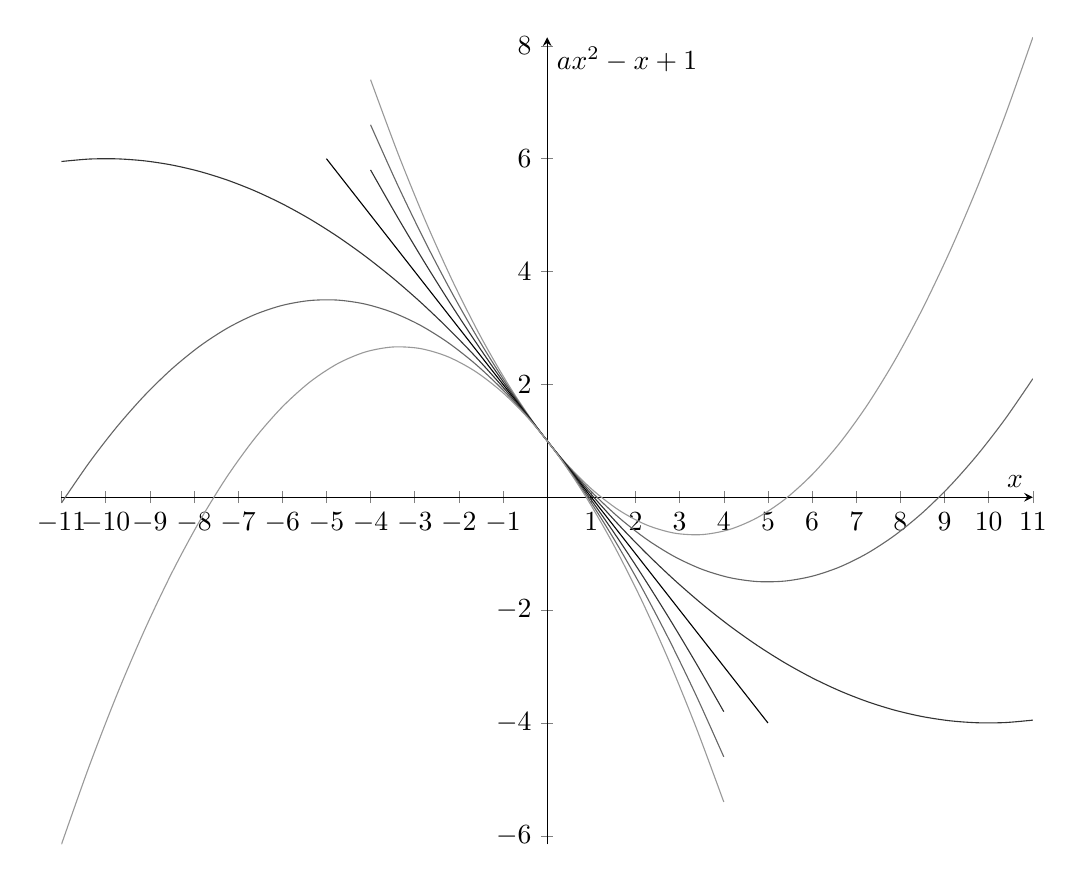
\begin{tikzpicture}
            \begin{axis} [
                scale=1.8,
                axis lines=center,
                xlabel={\(x\)},
                ylabel={\(ax^2 - x + 1\)},
                xtick distance=1]
                \addplot [domain=-4:11, smooth, black!40] { (0.15 * x^2) - x + 1 };
                \addplot [domain=-4:11, smooth, black!60] { (0.10 * x^2) - x + 1 };
                \addplot [domain=-4:11, smooth, black!80] { (0.05 * x^2) - x + 1 };
                \addplot [domain=-5:5, smooth, black] { (0.00 * x^2) - x + 1 };
                \addplot [domain=-11:4, smooth, black!80] { (-0.05 * x^2) - x + 1 };
                \addplot [domain=-11:4, smooth, black!60] { (-0.10 * x^2) - x + 1 };
                \addplot [domain=-11:4, smooth, black!40] { (-0.15 * x^2) - x + 1 };
            \end{axis}
        \end{tikzpicture}
    \end{center}
\end{solution}

\begin{problem}
    Find all real solutions of \(\para{4x^3 - 3x}^{2\sin\pi x} = 1\).
\end{problem}

\begin{solution}
    We may utilise the fact that \(a^b = 1\) if and only if \(a = 1\), or \(a \neq 0\) and \(b = 0\), or \(a = -1\) and \(b\) is even.

    We consider the following casework.

    \begin{itemize}
        \item \emph{\(4x^3 - 3x = 1\).} Notice \(x = 1\) is a solution, and hence
        \[
            4x^3 - 3x - 1 = \para{x - 1} \para{4x^2 + 4x + 1} = \para{x - 1} \para{2x + 1}^2
        \]
        so \(4x^3 - 3x = 1\) solves to \(x = 1\) or \(x = - \frac{1}{2}\).

        \item \emph{\(4x^3 - 3x \neq 0\) and \(2 \sin \pi x = 0\).} Note \(\sin \pi x = 0\) if and only if \(x \in \ZZ\), and \(4x^3 - 3x = 0\) if and only if \(x = 0\) or \(x = \pm \frac{\sqrt{3}}{2}\). Hence, this solves to \(x \in \ZZ, x \neq 0\).
        
        \item \emph{\(4x^3 - 3x = -1\) and \(2 \sin \pi x\) is even.} Note \(x = -1\) is a solution to \(4x^3 - 3x = -1\), and hence
        \[
            4x^3 - 3x + 1 = \para{x + 1}{4x^2 - 4x + 1} = \para{x - 1} \para{2x - 1}^2
        \]
        so \(4x^3 - 3x = -1\) solves to \(x = 1\) or \(x = \frac{1}{2}\).

        Note that they both satisfy \(2 \sin \pi x\) is even.
    \end{itemize}

    Therefore, the solutions are \(x \in \ZZ\) and \(x \neq 0\), or \(x = \pm \frac{1}{2}\).
\end{solution}

\subsection{Inequalities}

\begin{problem}
    Suppose that we have some positive integers (not necessarily distinct) whose sum is \(100\). How large can their product be?
\end{problem}

\begin{solution}
    First, we notice that having \(4\) in the optimal case is equivalent to having two \(2\)s, so we break them down into \(2\)s.
    
    If we have anything at least \(5\) in the optimal case, breaking it down into two integers would produce a greater product.
    
    If we have a \(1\) in the optimal case, it cannot be on its own, then combining it with any other integer \(n\) to get \(\para{n + 1}\) would give a greater product.

    Hence, the optimal product must (essentially) only contain \(2\)s and \(3\)s. But notice \(3^2 = 9 > 8 = 2^3\), so there has to be at most two \(2\)s in the optimal case (since if we have at least three \(2\)s, converting it into \(3\)s would produce a bigger product).

    Since \(100 = 3 \times 32 + 2 \times 2\), the greatest product must be
    \[
        2^2 \times 3^{32}.
    \]
\end{solution}